\documentclass[11pt]{article}
\input{\string~/.macros}
\usepackage[a4paper, total={7in, 9in}]{geometry}
\usepackage{bbm}
\usepackage{mathrsfs} % really cursive alphabets
\usepackage{graphicx}
    \graphicspath{{./assets}}
\usepackage{hyperref}
    \hypersetup{colorlinks=true, linktoc=all, linkcolor=blue, citecolor=red}
\usepackage[backend=bibtex,sorting=none]{biblatex}
\usepackage[margin=0cm]{caption}

% random variables
\newcommand\ry{\ensuremath{\mathsf{y}}}
\newcommand\rx{\ensuremath{\mathsf{x}}}
\newcommand\rb{\ensuremath{\mathsf{b}}} 
\newcommand\rc{\ensuremath{\mathsf{c}}}
\newcommand\rz{\ensuremath{\mathsf{z}}}
\newcommand\ru{\ensuremath{\mathsf{u}}}
\newcommand\rw{\ensuremath{\mathsf{w}}}
\newcommand\rpa{\ensuremath{\mathsf{pa}}}
\newcommand\rU{\ensuremath{\mathsf{U}}}
\newcommand\rbx{\ensuremath{\mathsf{\mathbf{x}}}}
\newcommand\rby{\ensuremath{\mathsf{\mathbf{y}}}}
\newcommand\rbu{\ensuremath{\mathsf{\mathbf{u}}}}

\newcommand\bbP{\ensuremath{\mathbbm{P}}}
\newcommand\bbQ{\ensuremath{\mathbbm{Q}}}


% boldsymbols
\renewcommand\bmu{\ensuremath{\boldsymbol{\mu}}}
\newcommand\bSigma{\ensuremath{\boldsymbol{\Sigma}}}
\newcommand\bgamma{\ensuremath{\boldsymbol{\gamma}}}
\newcommand\bomega{\ensuremath{\boldsymbol{\omega}}}
\newcommand\bnu{\ensuremath{\boldsymbol{\nu}}}


% optimization, classes of functions
\newcommand\scrF{\ensuremath{\mathscr{F}}}
\newcommand\scrS{\ensuremath{\mathscr{S}}}
\newcommand\scrP{\ensuremath{\mathscr{P}}}

% independence
\newcommand{\dperp}{\ensuremath{\perp\!\!\!\perp}}
\newcommand{\ndperp}{\ensuremath{\not\!\perp\!\!\!\perp}}

% operators
\newcommand{\prox}{\ensuremath{\mathsf{prox}}}
\addbibresource{GP.bib}
\addbibresource{multitask.bib}


\usepackage{tikz}
\newcommand*\circled[1]{\tikz[baseline=(char.base)]{
    \node[shape=circle, draw, inner sep=1pt, 
        minimum height=12pt] (char) {\vphantom{1g}#1};}}
\renewcommand\bf{\ensuremath{\mathbf{f}}} 



\begin{document}

 
\section{Gaussian Process}

\cite{carledwardrasmussenGaussianProcessMachine2006} introduces Gaussian Process regression as an alternative view to Bayesian regression. 

\subsection{Bayesian Regression}
 
In linear regression setup, we assume output $y\in\R$ is a linear function of inputs $x\in\R^d$, corrupted with additive iid normal noise,
\begin{align}
    y = f(x) + \epsilon
    \quad\text{where}\quad
    f(x) = w^Tx
    \quad\text{and}\quad
    \epsilon \sim \sN(0, \sigma_n^2)
\end{align}
The Bayesian setup considers $w\in\R^d$ as a random variable, endowed with prior $w\sim \sN(0,\Sigma_p)$. Using Bayes rule, we can find the posterior of weights given data, which is again a normal random variable $p(w \mid X, y) = \sN\left(w \; ; A^{-1}b, A^{-1} \right)$ where $A=\frac{1}{\sigma_n^2} X^TX + \Sigma_p^{-1}$ and $b = \frac{1}{\sigma_n^2}X^Ty$ and $X\in\R^{n\times d}, y\in\R^{n\times 1}$ are design matrices. For test point $x_*$, the predictive distribution of $f_*=f(x_*)$ is the average likelihood of $f_*$ under model $f(x;w)$ with respect to posterior of $w$.
\begin{align}
    p(f_*\mid x_*, X, y)
        = \int p(f_*\mid x_*,w) p(w\mid X, y) \, dw
    \label{eq:kernel_bayesian_regression_predictive_distribution_integral}
\end{align}
We can think of the predictive distribution as a linear function $f_* = x_*^Tw$ of weights, a normal random variable, and therefore is normal. Therefore, $f_*\mid x_*,X,y \sim \sN( x_*^T A^{-1}b, x_*^T A^{-1}x_* )$. The natural extension to Bayesian linear regression is to kernelize it, for example assume a linear model in some feature space $f(x) = \phi(x)^Tw$ for some feature map $\phi:\R^d\to\R^D$. We can write predictive distribution as 
\begin{align}
    f_* \mid x_*,X,y \sim \sN(
        & k(x_*,X) (k(X,X)+\sigma_n^2 I)^{-1}y, \\
        & k(x_*,x_*) - k(x_*,X)(k(X,X) + \sigma_n^2 I)^{-1} k(X,x_*))
    \label{eq:kernel_bayesian_regression_predictive_distribution}
\end{align}
where $k(X,X') = \Phi \Sigma_p \Phi'^T \in \R^{n\times n'}$ and $\Phi\in\R^{n\times D}$ are the feature vectors.

\subsection{Gaussian Process}


\begin{definition}
    (Gaussian Process) A Gaussian process is a stochastic process $\pc{X_t}_{t\in T}$ such that, for every finite subset of indices $t_1,\cdots,t_k \in T$, $(X_{t_1},\cdots,X_{t_k})$ is multivariate normal.
\end{definition}

A Gaussian process $f\sim \sG\sP(m,k)$ over $\R^{\sX}$ is fully specified by the mean function $m:\sX\to\R$ and covariance function $k:\sX\times\sX\to\R$ where
\begin{align}
    m(x)=\E\pb{f(x)}
    \quad\quad\quad
    k(x,x') = \E\pb{ (f(x)-m(x))(f(x')-m(x')) }
\end{align}
The covariance function determines function's behavior, for example its stationarity, smoothness, and periodicity etc. For example, the squared exponential covariance function $k_{\text{SE}}(x,x') = \exp( -\frac{1}{2\ell^2} \norm{x-x'}_2^2 )$ enforces the prior knowledge that functions are smooth, i.e. inputs are close in the Euclidean sense will have similar outputs. See Figure (\ref{fig:plt_sample_from_gp}) for some examples of samples from Gaussian process.

\begin{example}
    (Intuition about covariance matrix for $\sG\sP$) First consider $(y_1,y_2) \sim \sN(\mathbf{0}, \Sigma)$ where $\Sigma_{11}=\Sigma_{22} = 1$ and $\Sigma_{12}=\Sigma_{21}=\rho_{12}$. We know $y_1\mid y_2 = a \sim \sN(\rho_{12} a, 1 -  \rho_{12}^2)$. When $\cov(y_1,y_2) = \rho_{12} \uparrow 1$, $y_1$'s samples conditioned on $y_2=a$ fall close to $a$ with high probability. When $\rho_{12} \downarrow 0$, $y_1 \mid y_2=a$ will distribute like a unit normal, regardless of values that $y_2$ take. Extend this intuition to gaussian process: whenever $k(x_i,x_j)$ is large, $y_i,y_j$ are correlated and so observing $y_i=a$ provides a strong prior on how $y_j$ will behave, or in other words, reduce the uncertainty of values that $y_j$ can take dramatically.
\end{example}


\begin{center} 
\begin{figure}[h!]
    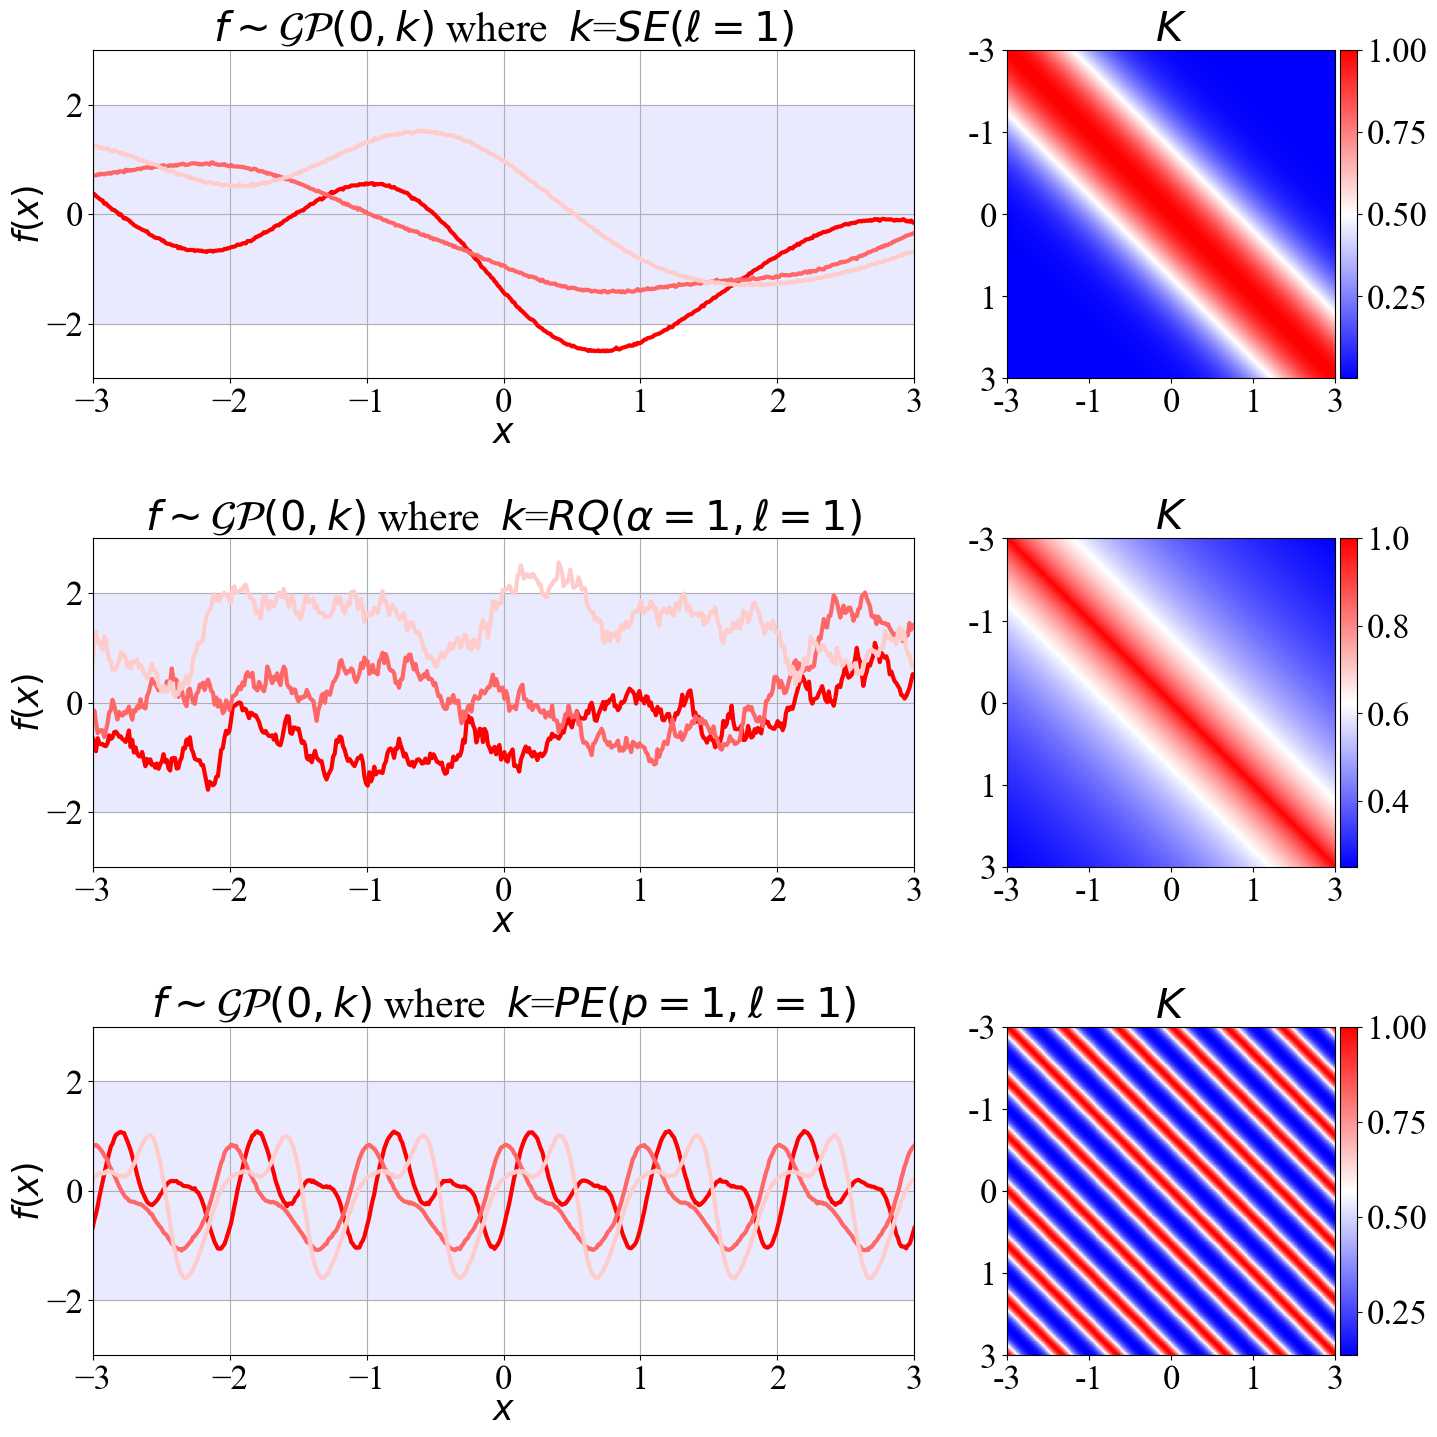
\includegraphics[width=\textwidth]{assets/plt_sample_from_gp.png} 
    \caption{(Left) Samples from Gaussian process prior and (Right) covariance matrix at test locations.}
    \label{fig:plt_sample_from_gp}
\end{figure}
\end{center} 
    

\subsection{Gaussian Process Regression}

Instead of placing a prior over weights $p(w)$ to quantify randomness in function $f(x)=\phi(x)^Tw$, we model function directly as a Gaussian process, $f\sim \sG\sP(0,k)$. There is a one-to-one correspondence between the two views. For example, $f(x)=\phi(x)^Tw$ with prior $w\sim \sN(0,\Sigma_p)$ used in kernel Bayesian regression has
\begin{align}
    \E\pb{f(x)}
        = \phi(x)^T \E\pb{w} = 0
    \quad\quad\quad
    \E\pb{ f(x)f(x') }
        = \phi(x)^T\Sigma_p \phi(x')
\end{align}
Therefore, $f\sim \sG\sP(0, k)$ where $k(x,x') = \phi(x)^T \Sigma_p \phi(x')$. Note $k$ is in fact a valid kernel. (Since $\Sigma_p$ is psd, $\Sigma_p = UDU^T$ by SVD. We can write $k(x,x') = \inner{\psi(x)}{\psi(x')}$ where $\psi(x) = \Sigma_p^{1/2} \phi(x)$ and $\Sigma_p^{1/2} = UD^{1/2}U^T$). Conversely, any valid kernel used in kernel Bayesian regression can be used to parameterize the covariance function of the Gaussian process model over $f$.

Since $y=f(x)+\epsilon$, we have $\by = \bf + \sigma_n^2 I \sim \sN(0, k(X,X)+\sigma_n^2I)$ where $\by,\bf\in\R^{n\times 1}$. We can write the joint distribution of observed values and function values at some test locations $X_*$ as
\begin{align}
    \begin{bmatrix}
        \by \\ \bf_*
    \end{bmatrix}
    \sim
    \sN\left(
        \mathbf{0},
        \begin{bmatrix}
            k(X,X) + \sigma_n^2I & k(X,X_*) \\
            k(X_*,X) & k(X_*,X_*) \\ 
        \end{bmatrix}
    \right)
    \label{eq:gaussian_process_regression_noisy_model}
\end{align}
We can derive the predictive distribution for $\bf_*\mid \by$ by simply apply conditional distribution formula
\begin{align}
    \bf_* \mid X,\by, X_* \sim \sN(
        & k(X_*,X) (k(X,X)+\sigma_n^2 I)^{-1} \by  \\
        & k(X_*,X_*) - k(X_*,X) (k(X,X)+\sigma_n^2 I)^{-1} k(X,X_*) )
    \label{eq:gp_regression_predictive_distribution}
\end{align}
which has exact form compared to (\ref{eq:kernel_bayesian_regression_predictive_distribution}). More compactly, for a single test point $x_*$, $\mu_{\bf_*} =  k_*^T (K+\sigma_n^2 I)^{-1}$ and $\var(\bf_*) = k(x_*,x_*) - k_*^T (K+\sigma_n^2 I)^{-1} k_* $ where $k_* = k(X,x_*)\in \R^{n\times 1}$. See Figure (\ref{fig:plt_gp_regression_inference}) for examples of Gaussian process regression with varying data size and hyperparameters. 

 
\begin{center} 
\begin{figure}[h!]
    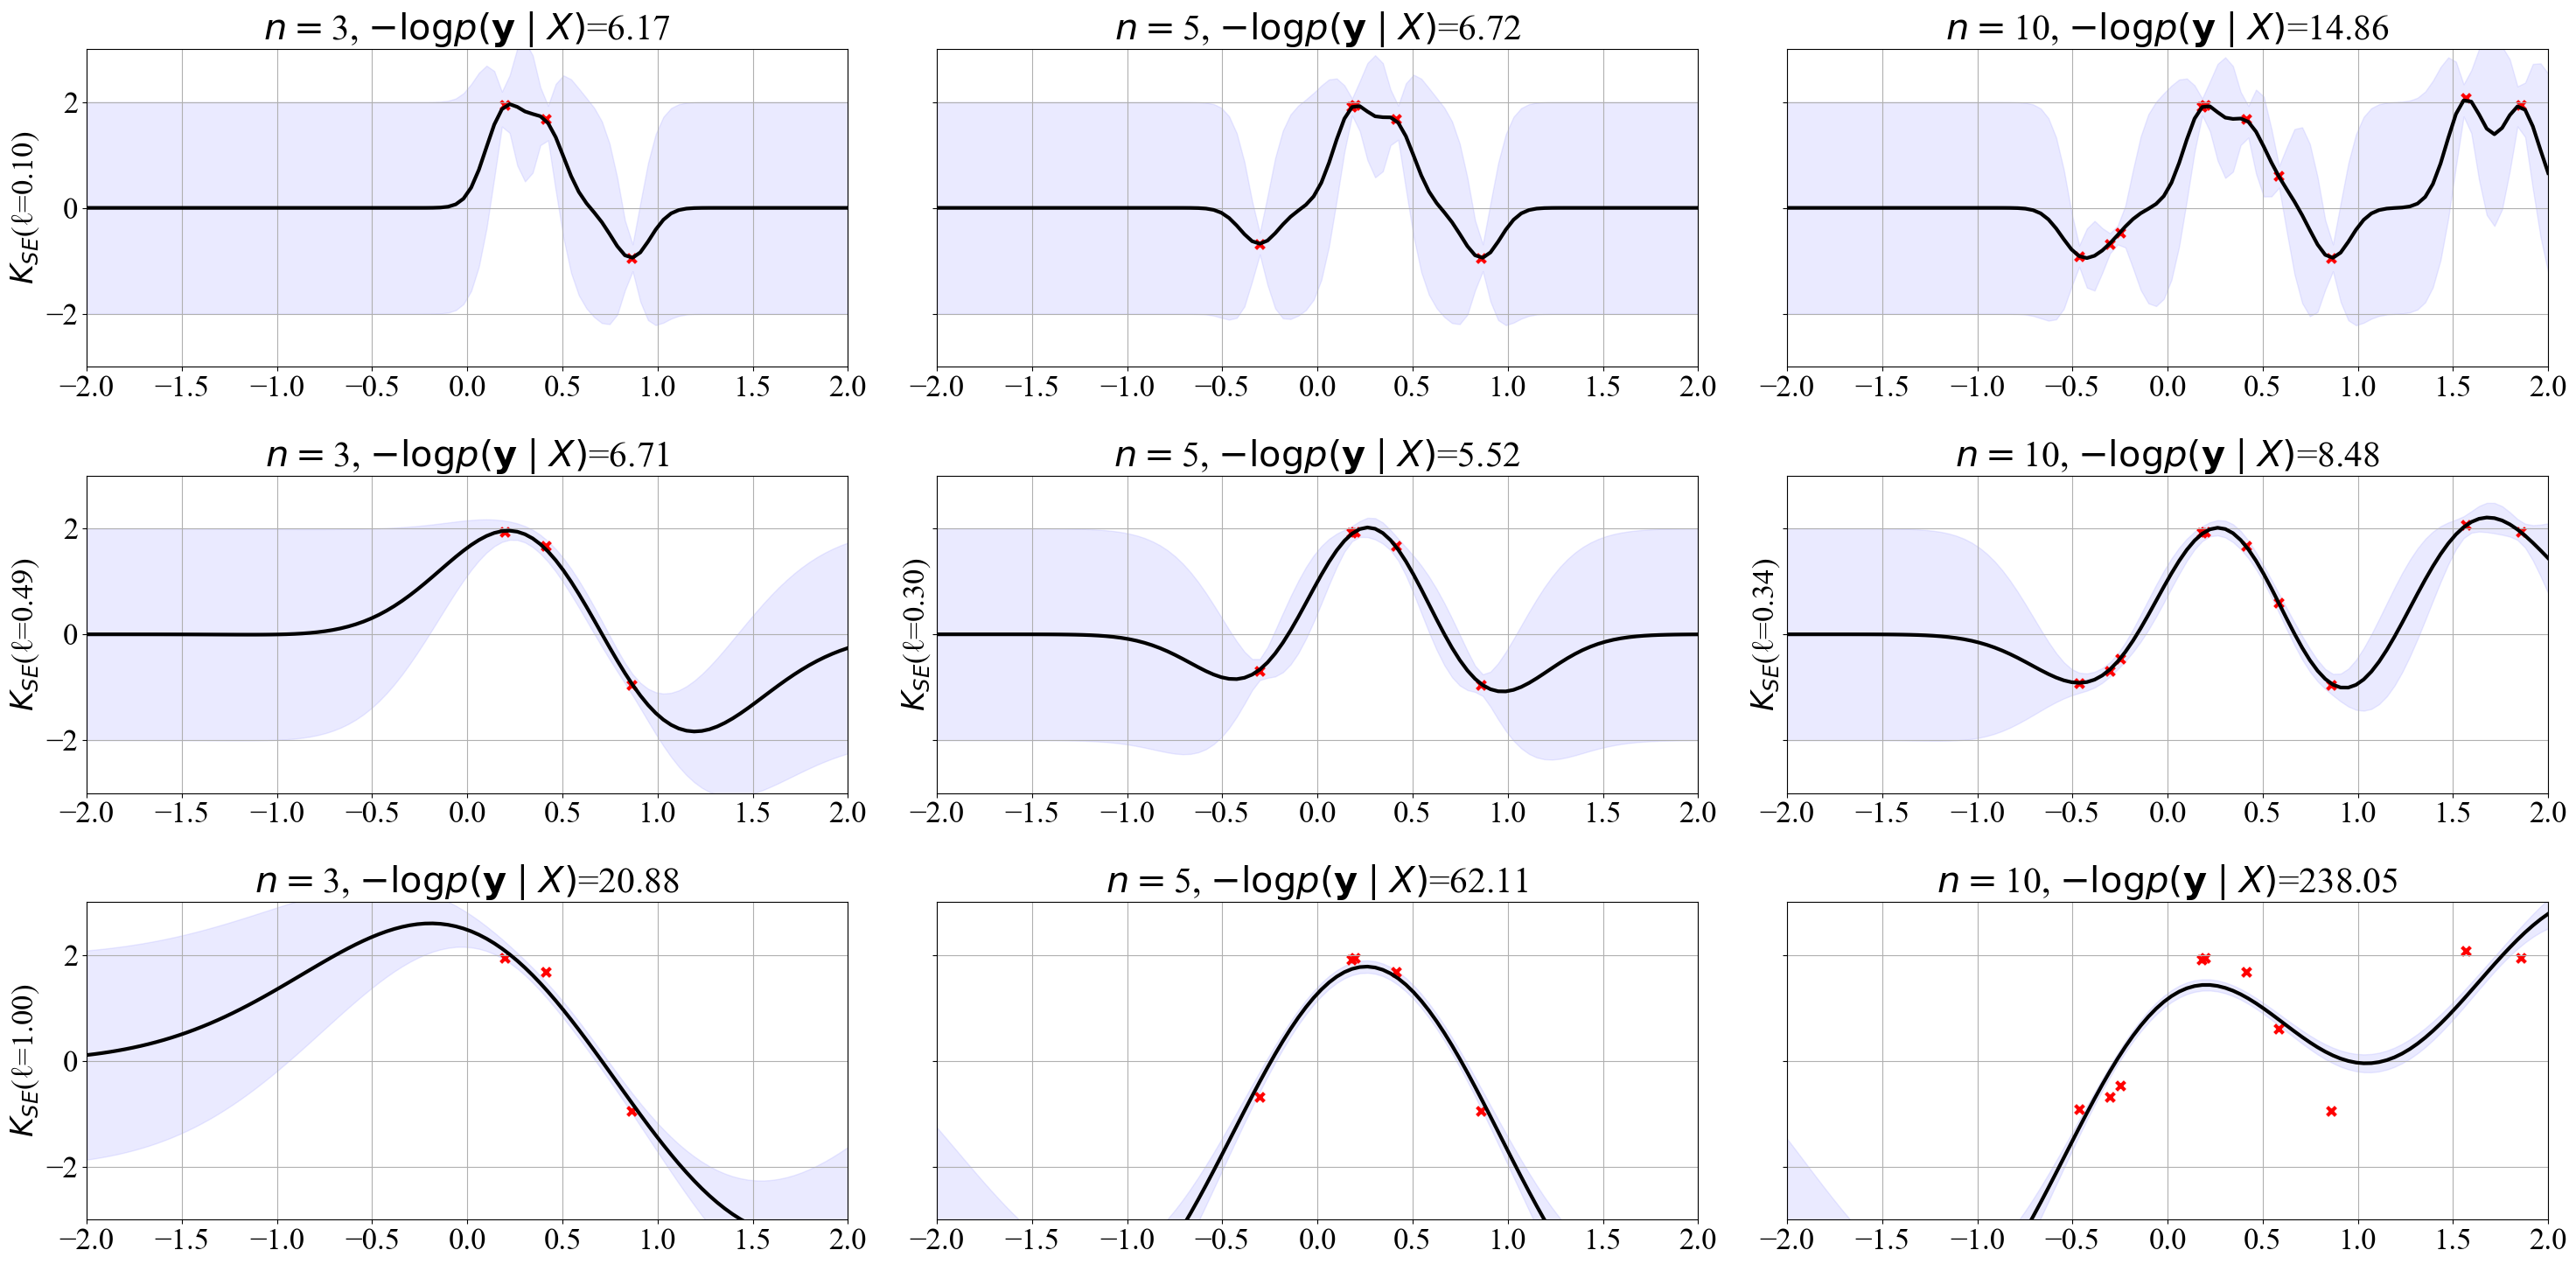
\includegraphics[width=\textwidth]{assets/plt_gp_regression_inference.png} 
    \caption{This plot shows mean (black) and 95\% confidence interval (light blue) for predictive distribution $p(\bf_*\mid X,\by, X_*)$ fit using Gaussian process regression assuming a SE prior over $f\sim\sG\sP(0,k_{SE})$ of varying lengthscale $\ell$ and observed sample sizes $n$ given groundtruth noise $\sigma_n=0.3$. The middle row's hyperparameters is taken to be the empirical Bayes estimate $\ell,\sigma_n = \argmax p(\by\mid X, \ell,\sigma_n)$ where $p(\by\mid X,\ell,\sigma_n)$ given by Equation (\ref{eq:gp_regression_marginal_likelihood}), optimized via gradient descent. Note estimating $\log(\ell),\log(\sigma_n)$ makes the optimization problem much easier.}
    \label{fig:plt_gp_regression_inference}
\end{figure}
\end{center}

\subsection{Model Selection}

Model selection for Gaussian process regression involves picking the form and the hyperparameters of the covariance function. Given data $(X,\by)$, marginal likelihood $p(\by\mid X)$ quantifies how likely data is observed under our additive noise model $\by\mid \bf \sim \sN(\bf,\sigma_n^2 I)$ on average with respect to latent function values (or parameters of our model) $\bf\mid X \sim \sN(0,K)$ (due to assumption of Gaussian process prior over f),
\begin{align}
    p(\by\mid X)
        = \int p(\by\mid \bf,X) p(\bf\mid X) \, d\bf
\end{align}
This formulation is analogous to that in Bayesian linear regression where the marginal likelihood marginalizes over weights $p(\by\mid X) = \int p(\by\mid X,w)p(w) \, dw$. We can obtain a closed form expression by reading off (\ref{eq:gaussian_process_regression_noisy_model}), i.e. $\by \sim \sN(\mathbf{0}, K+\sigma_n^2 I)$. 
\begin{align}
    \log p(\by\mid X)
        = -\frac{1}{2} \by^T  (K+\sigma_n^2 I)^{-1}\by - \frac{1}{2} \log |K+\sigma_n^2I| - \frac{n}{2} \log 2\pi 
    \label{eq:gp_regression_marginal_likelihood}
\end{align}
In Bayesian model selection, model hyperparameters for Gaussian process regression $\theta = \pc{\sigma_n, \ell}$ can be found by maximizing the marginal likelihood or the type II likelihood $\theta^* = \argmax_{\theta}\, \log p(\by\mid X, \theta)$.





\section{Approximate Gaussian Process}

\subsection{Inducing Variables (DIC/FITC)}

The unifying view paper \cite{quinonero-candelaUnifyingViewSparse2005} gives a pretty good explanation/interpretation of sparse GP methods based on inducing points till circa 2005. The basic idea is to augment existing model $p(\by,\bf)$ with $m$ additional inducing variables $\bu = \pc{u}_{i=1}^m$ that are instantiation from the same GP prior, corresponding to a set of inducing locations $X_{\bu}$. Inducing variables act as an information channel between training/testing latent function values $\bf,\bf_*$, alternatively we can think of $\bu$ as a sufficient statistics of potentially redundant latent function values $\bf$. This translates to a conditional independence assumption $\bf \dperp \bf_* \mid \bu$, which implies the following factorization,
\begin{align}
    p(\by\mid\bf)p(\bf,\bf_*,\bu)
        = p(\by\mid\bf) p(\bf\mid \bu) p(\bf_*\mid \bu) p(\bu)
\end{align}
Without additional assumptions, we can think of joint priors factorizes akin to a latent variable model,
\begin{align}
    \bu
        &\sim \sN(0, K_{\bu\bu}) \\ 
    \bf\mid\bu
        &\sim \sN( K_{\bf\bu}K_{\bu\bu}^{-1} \bu, K_{\bu\bu} - Q_{\bf\bf} ) 
    \label{eq:inducing_variables_conditional_prior}
\end{align}
where $Q_{\bf\bf}=K_{\bf\bu}K_{\bu\bu}^{-1}K_{\bu\bf}$ is Nystr\"om approximation of $K_{\bf\bf}$. Various approximation schemes corresponds to approximations to the conditional prior, $q(\bf\mid \bu), q(\bf_* \mid \bu)$. For exact GP, inference using the posterior GP $p(\bf\mid\by)$ requires inversion of a large kernel matrix; The introduction of inducing variables modifies the form that posterior GP $q(\bf\mid\by)$ takes.

To start, the Subset of Regressor (SoR) or Deterministic Inducing Conditional (DIC) approximation assumes that the latent function values as a linear mapping of inducing variables, e.g. $\bf = K_{\bf\bu} K_{\bu\bu}^{-1} \bu$. Note that the linear projection is one which preserves the mean of conditional prior in Equation (\ref{eq:inducing_variables_conditional_prior}). This assumption gives to an approximate conditional prior with zero covariance, $q_{\text{SOR}}(\bf\mid\bu) = \sN(  K_{\bf\bu} K_{\bu\bu}^{-1} \bu, 0 )$. Because of the linear mapping, $\E_q\pb{\bf} = 0$ and $\cov_q(\bf) = K_{\bf\bu}K_{\bu\bu}^{-1} K_{\bu\bu} K_{\bu\bu}^{-1} K_{\bu\bf} = Q_{\bf\bf}$, similarly for $q(\bf_*)$, and therefore,
\begin{align}
    q_{\text{DIC}}(\bf,\bf_*)
        = \sN\left( 0,
            \begin{bmatrix}
                Q_{\bf\bf} & Q_{\bf*} \\
                Q_{\bf*} & Q_{**} \\ 
            \end{bmatrix}
        \right)
\end{align}
Inference with the DIC approximation is equivalent to exact inference with a modified covariance function $k_{\text{DIC}}(x_i,x_j) = k(x_i, \bu) K_{\bu\bu}^{-1} k(\bu, x_j)$. The predictive distribution is then given by 
\begin{align}
    q_{\text{DIC}}(\bf_*\mid \by)
        \sim \sN\left(
            Q_{*\bf} ( Q_{\bf\bf} + \sigma_n^2 I )^{-1} \by,
            Q_{**} - Q_{*\bf} ( Q_{\bf\bf} + \sigma_n^2 I )^{-1} Q_{\bf*}
        \right)
\end{align}
Inversion of a $n\times n$ matrix is replaced with inversion of $m\times m$ matrix, making computation faster. 

Sparse Gaussian Process using Pseudo-inputs (SGPP) or Fully Independent Training Conditional (FITC) approximation is another popular approximate GP method \cite{snelsonSparseGaussianProcesses2005}. Simply, FITC assumes $\bf_i\dperp \bf_j \mid \bu$ for all $i,j\in\pb{n}$, henceforth the conditional priors are fully (conditionally) independent. 
\begin{align}
    q_{\text{FITC}}(\bf\mid\bu)
        = \prod_{i=1}^n p(f_i\mid \bu)
        = \sN( K_{\bf\bu}K_{\bu\bu}^{-1} \bu, \text{diag}\pb{ K_{\bu\bu} - Q_{\bf\bf} } )
\end{align}
Compare this to Equation (\ref{eq:inducing_variables_conditional_prior}), we see that FITC replaces approximate covariances with exact covariances on the diagonal. Equivalently, we can think of $\bf$ as a noisy linear map of $\bu$ where the noise has a particular form, e.g. $\bf = K_{\bf\bu}K_{\bu\bu}^{-1} \bu + \gamma$ where $\gamma \sim \sN(0, \text{diag}\pb{ K_{\bu\bu} - Q_{\bf\bf} })$. We can derive the covariance for the approximate posterior $\cov_q(\bf) = \cov( K_{\bf\bu}K_{\bu\bu}^{-1} \bu ) + \cov( \gamma ) = Q_{\bf\bf} + \text{diag}\pb{  K_{\bu\bu} - Q_{\bf\bf} }$. Therefore,
\begin{align}
    q_{\text{FITC}}(\bf,\bf_*)
        = \sN\left(
            0,
            \begin{bmatrix}
                Q_{\bf\bf} - \text{diag}\pb{Q_{\bf\bf} - K_{\bf\bf}} & Q_{\bf*} \\ 
                Q_{*\bf} & K_{**} \\
            \end{bmatrix}
        \right)
\end{align}
Inference with FITC approximation is equivalent to exact inference with a modified covariance function $k_{\text{FITC}}(x_i,x_j) = k_{\text{DIC}}(x_i,x_j) + \delta_{i,j} (k(x_i,x_j) - k_{\text{DIC}}(x_i,x_j))$. The predictive distribution follows,


\begin{align}
    q_{\text{FITC}}(\bf_*\mid \by)
        &\sim \sN\left(
            Q_{*\bf} ( Q_{\bf\bf} + \Lambda )^{-1} \by,
            K_{**} - Q_{*\bf} ( Q_{\bf\bf} + \Lambda )^{-1} Q_{\bf*}
        \right) 
        \label{eq:fitc_predictive_intuitive}
        \\
        &\sim \sN\left(
            K_{*\bu}\Sigma K_{\bu\bf} \Lambda^{-1} \by,
            K_{**} - Q_{**} + K_{*\bu}\Sigma K_{\bu*}
        \right)
        \label{eq:fitc_predictive_computation}
\end{align}
where $\Lambda = \text{diag}\pb{ K_{\bf\bf} - Q_{\bf\bf} + \sigma_n^2 I }$ and $\Sigma = (K_{\bu\bu} + K_{\bu\bf}\Lambda^{-1}K_{\bf\bu})^{-1}$. Here Equation (\ref{eq:fitc_predictive_intuitive}) follows from natural derivation and the Equation (\ref{eq:fitc_predictive_computation}) is more computationally attractive. To see the equivalence, we first apply Woodbury inversion formula,
\begin{align}
    (\Lambda + Q_{\bf\bf})^{-1}
        = \Lambda^{-1} - \Lambda^{-1} K_{\bf\bu} (K_{\bu\bu} + K_{\bu\bf} \Lambda^{-1} K_{\bf\bu} )^{-1} K_{\bu\bf} \Lambda^{-1}
    \label{eq:fitc_woodbury_inverse}
\end{align}
By definition of $\Sigma$, we have $(\Lambda + Q_{\bf\bf})^{-1} = \Lambda^{-1} - \Lambda^{-1} K_{\bf\bu} \Sigma K_{\bu\bf} \Lambda^{-1}$. Therefore,
\begin{align*}
    \mu_{\bf_*} 
        &= Q_{*\bf} ( Q_{\bf\bf} + \Lambda )^{-1} \by  \\
        &= K_{*\bu} K_{\bu\bu}^{-1} K_{\bu*} ( \Lambda^{-1} - \Lambda^{-1} K_{\bf\bu} \Sigma K_{\bu\bf} \Lambda^{-1} ) \by 
            \tag{Woodbury with defn $\Sigma$} \\
        &= K_{*\bu} K_{\bu\bu}^{-1} ( \Sigma^{-1} - K_{\bu\bf} \Lambda^{-1} K_{\bf\bu} ) \Sigma K_{\bu\bf} \Lambda^{-1} \by 
            \tag{pull out $\Sigma K_{\bu\bf}\Lambda^{-1}$}
        \\
        &= K_{*\bu} K_{\bu\bu}^{-1} K_{\bu\bu} \Sigma K_{\bu\bf} \Lambda^{-1} \by
            \tag{defn $\Sigma$} \\
        &= K_{*\bu}\Sigma K_{\bu\bf} \Lambda^{-1} \by \\
    \cov_{\bf_*}
        &= K_{**} - Q_{*\bf} ( Q_{\bf\bf} + \Lambda )^{-1} Q_{\bf*} \\ 
        &= K_{**} - K_{*\bu}\Sigma K_{\bu\bf} \Lambda^{-1} K_{\bf\bu} K_{\bu\bu}^{-1} K_{\bu*} 
            \tag{results from $\mu_{\bf_*}$} \\
        &= K_{**} - K_{*\bu}\Sigma (\Sigma^{-1} - K_{\bu\bu}) K_{\bu\bu}^{-1} K_{\bu*} 
            \tag{defn $\Sigma$} \\
        &= K_{**} - Q_{**} + K_{*\bu}\Sigma K_{\bu*}
\end{align*}


One popular methods for selecting inducing inputs $\bX_u$ is simply by maximizing the marginal likelihood
\begin{align}
    q(\by\mid X_{\bu})
        = \iint p(\by\mid \bf) q(\bf\mid \bu) p(\bu\mid X_{\bu}) \, d\bu \, d\bf
\end{align}


\subsection{Implementation Details}

To optimize for inducing variables, we need a computationally stable way to compute $\log p(\by\mid X)$. More specifically, we need a way to compute $\by^T (\Lambda + Q_{\bf\bf})^{-1} \by$ and $\log | \Lambda + Q_{\bf\bf} |$. Referencing (\href{https://github.com/GPflow/GPflow/blob/develop/gpflow/models/sgpr.py#L263}{gpflow}, \href{https://bwengals.github.io/pymc3-fitcvfe-implementation-notes.html}{a blog}),
\begin{align*}
    (\Lambda + Q_{\bf\bf})^{-1}
        &= (\Lambda + V^TV)^{-1}
            \tag{\texttt{chol} $K_{\bu\bu} = L_{\bu\bu} L_{\bu\bu}^T$, \texttt{backsolve} $V = L_{\bu\bu}^{-1}K_{\bu\bf}$, $Q_{\bf\bf} = V^TV$} \\ 
        &= \Lambda^{-1} - \Lambda^{-1} V^T (I + V\Lambda^{-1}V^T)^{-1} V \Lambda^{-1}
            \tag{Woodbury} \\
        &= \Lambda^{-1} - \Lambda^{-1} V^T L_B^{-T} L_B^{-1} V \Lambda^{-1}
            \tag{$B:= I + V\Lambda^{-1}V^T$, \texttt{chol} $B = L_{B}L_{B}^T$} \\
    \by^T (\Lambda + Q_{\bf\bf})^{-1} \by
        &= \by^T \Lambda^{-1} \by - \bgamma^T\bgamma
            \tag{\texttt{backsolve} $\bgamma = L_B^{-1} V\Lambda^{-1} \by $}  \\
    \log \det (\Lambda + Q_{\bf\bf})
        &= \log \det(I + V\Lambda^{-1}V^T) + \log \det(\Lambda)
            \tag{ Matrix inversion lemma, $Q_{\bf\bf} = V^TV$} \\ 
        &= \log \det(B) + \log \det(\Lambda)  
            \tag{defn $B$} \\
        &= 2\log \det(L_B) + \log \det(\Lambda)
\end{align*}
Put everything together, we have an expression that involves mostly $\sO(m^3)$ \texttt{chol} and $\sO(nm^2)$ \texttt{backsolve},
\begin{align}
    \log p(\by\mid X)
        = - \frac{1}{2} \by^T \Lambda^{-1} \by + \frac{1}{2} \bgamma^T\bgamma - \sum_{i=1}^m \log \pb{L_B}_{ii} -\frac{1}{2} \sum_{i=1}^n \log \pb{\Lambda}_{ii} - \frac{n}{2} \log(2\pi)
\end{align}
We can also compute the predictive distribution in Equation (\ref{eq:fitc_predictive_computation}) as follows,
\begin{align*}
    \Sigma
        &= (K_{\bu\bu} + K_{\bu\bf}\Lambda^{-1}K_{\bf\bu})^{-1} \\
        &= (L_{\bu\bu} L_{\bu\bu}^T + L_{\bu\bu} L_{\bu\bu}^{-1} K_{\bu\bf}\Lambda^{-1}K_{\bf\bu} L_{\bu\bu}^{-T} L_{\bu\bu}^T ) 
            \tag{$K_{\bu\bu} = L_{\bu\bu} L_{\bu\bu}^T$} \\
        &= (L_{\bu\bu} B L_{\bu\bu}^T)^{-1}
            \tag{$B = I + L_{\bu\bu}^TL_{\bu\bf} \Lambda^{-1} K_{\bf\bu} L_{\bu\bu}^{-T}$} \\
        &= L_{\bu\bu}^{-T} L_{B}^{-T} L_{B}^{-1} L^{-1} \\
    \mu_{\bf_*}
        &= K_{*\bu}\Sigma K_{\bu\bf} \Lambda^{-1} \by \\ 
        &= K_{*\bu}  L_{\bu\bu}^{-T} L_{B}^{-T} L_{B}^{-1} L^{-1} K_{\bu\bf} \Lambda^{-1} \by 
            \tag{ substitute $\Sigma$} \\
        &= K_{*\bu}  L_{\bu\bu}^{-T} L_{B}^{-T} \bgamma
            \tag{ $\bgamma = L_B^{-1}L_{\bu\bu}^{-1} K_{\bu\bf} \Lambda^{-1}\by $} \\
        &= \bomega^T L_{B}^{-T} \bgamma 
            \tag{\texttt{backsolve} $\bomega = L_{\bu\bu}^{-1} K_{\bu *}$ implies $Q_{**}=\bomega^T\bomega$} \\
    \cov_{\bf_*}
        &= K_{**} - Q_{**} + K_{*\bu}\Sigma K_{\bu*} \\
        &= K_{**} - Q_{**} + K_{*\bu} L_{\bu\bu}^{-1} L_B^{-1} L_B^{-1} L_{\bu\bu}^{-1} K_{\bu *} 
            \tag{substitute $\Sigma$} \\
        &= K_{**} - \bomega^T \bomega + \bnu^T \bnu 
            \tag{\texttt{backsolve} $\bnu = L_B^{-1} \bomega$}
\end{align*}
Note that there are two additional \texttt{backsolve} to compute the predictive distribution.





\subsection{Variational Formulation (VFE/SVGP)}


Sparse GP with inducing variables is inflicted with the problem that modeling assumptions, e.g. choice of covariance function, is interwined with approximation assumptions. Specifically, we see that inference using approximation schemes like DIC and FITC can be interpreted as performing exact inference on GP model with a modified covariance function, where inducing locations $X_{\bu}$ are part of kernel hyperparameters. This is undesirable.

\cite{titsiasVariationalLearningInducing2009} proposes to use variational inference to learning inducing locations. \cite{hensmanGaussianProcessesBig2013} extends the variational bound for stochastic gradient optimization, \cite{hensmanScalableVariationalGaussian2014} extends the variational bound to account for non-conjugate likelihood. The accompanying technical report for the 2009 paper \cite{titsiasVariationalModelSelection2009}, the gentle tutorial \cite{galVariationalInferenceSparse2014}, another report by Thang Bui \cite{buiSparseApproximationsNonConjugate2014}, Mark van der Wilk's PhD thesis \cite{SparseGaussianProcess2018} are helpful in understanding the derivations.

\cite{titsiasVariationalLearningInducing2009} proposes Variational Free Energy (VFE) which applies variational inference to learn inducing variables in sparse GP, alleviating the above concern. Similar to inducing variable approximations, the model is augmented with inducing variables and assume the same conditional independence relationship so that the joint density factorizes $p(\by,\bf,\bu) = p(\by\mid\bf) p(\bf\mid \bu) p(\bu)$. Here $\by$ is observed while $\pc{\bu,\bf}$ are latent variables. In contrast to inducing variable methods which makes approximating assumptions about the conditional priors, the paper introduce a variational density that preserves the true conditional prior with a freely varying prior over the inducing variables, e.g. $q(\bf,\bu) = p(\bf\mid\bu)q(\bu)$ for some $q(\bu)\sim \sN(\mu_{\bu},\Sigma_{\bu})$ that depends on inducing locations $X_{\bu}$ as well as kernel hyperparameters. Together with Equation (\ref{eq:inducing_variables_conditional_prior}), we can derive an approximate posterior for $\bf$,
\begin{align}
    q(\bf)
        = \int p(\bf\mid\bu)q(\bu) \, d\bu
        = \sN( K_{\bf\bu} K_{\bu\bu}^{-1} \mu_{\bu},
               K_{\bf\bf} - Q_{\bf\bf} +  K_{\bf\bu} K_{\bu\bu}^{-1} \Sigma_{\bu} K_{\bu\bu}^{-1} K_{\bu\bf} )
    \label{eq:inducing_variables_approximate_prior_f}
\end{align}
The paper then proposes to find variational parameters $\pc{\mu_n,\Sigma_n,X_{\bu},\theta}$ by minimizing the distance between the approximate and true posterior, $q^* = \argmin_{q(\bu)} \text{KL}(q(\bf,\bu)\mid p(\bf,\bu\mid \by))$. As usual in variational inference, we derive the ELBO to make objective tractable for optimization,
\begin{align}
    \text{KL}(q(\bf,\bu)\mid p(\bf,\bu\mid \by))
        &= \int p(\bf\mid\bu) q(\bu) \log \left( \frac{p(\bf\mid\bu)q(\bu)}{p(\by\mid\bf) p(\bf\mid\bu) p(\bu)}  \right) \, d\bf\, d\bu + \log p(\by) \\
    \log p(\by)
        &\geq \int q(\bu) \int p(\bf\mid\bu) \log p(\by\mid \bf) \, d\bf \, d\bu - \text{KL}(q(\bu) \Vert p(\bu))
    \label{eq:sparse_gp_vfe_elbo}
\end{align}
With $\E\pb{\bf\mid\bu} = K_{\bf\bu} K_{\bu\bu}^{-1}\bu$ and $\cov(\bf\mid\bu) = K_{\bf\bf} - Q_{\bf\bf}$, we can simplify,
\begin{align}
    \langle \log p(\by\mid\bf) \rangle_{p(\bf\mid\bu)}
        &= \int p(\bf\mid\bu) \pb{
            -\frac{n}{2} \log(2\pi \sigma^2) - \frac{1}{2\sigma^2} \tr\left( \by\by^T - 2\by\bf^T + \bf\bf^T \right)
        }\, d\bf \\
        &=  -\frac{n}{2} \log(2\pi \sigma^2) - \frac{1}{2\sigma^2} \tr\left( \by\by^T - 2\by (\E\pb{\bf\mid\bu})^T + \cov(\bf\mid\bu) + \E\pb{\bf\mid\bu} \E\pb{\bf\mid\bu}^T \right) \\
        &=  \log \sN(\bf \mid K_{\bf\bu}K_{\bu\bu}^{-1}\bu, \sigma^2I) - \frac{1}{2\sigma^2} \tr\left( K_{\bf\bf} - Q_{\bf\bf} \right)
\end{align}
Now with $P:= K_{\bf\bu}K_{\bu\bu}^{-1}$, $\E_q\pb{\bu} = \mu_{\bu}$, and $\cov_q(\bu) = \Sigma_{\bu} + \mu_{\bu}\mu_{\bu}^T$, then
\begin{align}
    \langle \log p(\by\mid \bf) \rangle_{q(\bf,\bu)}
        &=  -\frac{n}{2} \log(2\pi \sigma^2) - \frac{1}{2\sigma^2} \tr\left( \by\by^T - 2\by ( P \mu_{\bu})^T + P ( \Sigma_{\bu} + \mu_{\bu}\mu_{\bu}^T ) P^T + K_{\bu\bu} - Q_{\bu\bu} \right) \\
        &=  \log \sN(\bf \mid K_{\bf\bu}K_{\bu\bu}^{-1}\mu_{\bu}, \sigma^2I) - \frac{1}{2 \sigma^2} \tr\left( K_{\bf\bf} - Q_{\bf\bf} \right) - \frac{1}{2\sigma^2} \tr\left( K_{\bf\bu}K_{\bu\bu}^{-1} \Sigma_{\bu} K_{\bu\bu}^{-1} K_{\bu\bf} \right)
    \label{eq:sparse_gp_vfe_elbo_1}
\end{align}
\cite{titsiasVariationalLearningInducing2009} finds the optimal variational distribution $q(\bu)$ and substitute back into the lower bound, resulting in a bound where the first term is simply the marginal likelihoood for sparse GP with DIC approximation while the second term minimizes the error of predicting $\bf$ from $\bu$, e.g. $\tr(\cov(\bf\mid\bu)) = \min \E\norm{P \bu-\bf}_2^2$,
\begin{align}
    \sL_{\text{VFE}}
        :=  \log \sN(\bf \mid \mathbf{0},Q_{\bf\bf} +  \sigma^2I) - \frac{1}{2\sigma^2} \tr\left( K_{\bf\bf} - Q_{\bf\bf} \right)
    \label{eq:sparse_gp_vfe_collapsed_bound}
\end{align}
The bound is strictly better with additional inducing variables and becomes tight when $X_{\bu}=X$, recovering the full GP marginal likelihood. Maximizing $\sL_{\text{VFE}}$ with respect to kernel hyperparameters and inducing locations is tractable as the objective requires $\sO(nm^2)$ to compute.

\cite{hensmanGaussianProcessesBig2013} proposes Stochastic Variational Gaussian Process (SVGP) that extends the bound (\ref{eq:sparse_gp_vfe_elbo}) to allow for stochastic variational inference. The key obseration is that with $p(\by\mid\bf) = \prod_{i=1}^n p(y_i\mid f_i)$, the lower bound factors with respect to data points. Start with Equation (\ref{eq:sparse_gp_vfe_elbo}),
\begin{align}
    \log p(\by) 
        &\geq \langle \log p(\by\mid\bf) \rangle_{q(\bf)} - \text{KL}\left( q(\bu) \Vert p(\bu) \right) 
        = \sum_{i=1}^n \langle  \log p(y_i\mid f_i) \rangle_{q(f_i)} - \text{KL}\left( q(\bu) \Vert p(\bu) \right) \\
    \langle  \log p(y_i\mid f_i) \rangle_{q(f_i)}
        &= \langle -\frac{1}{2} \log (2\pi \sigma^2) - \frac{1}{2\sigma^2} (y_i^2 - 2y_if_i + f_i^2) \rangle_{q(f_i)} \\
        &=  -\frac{1}{2} \log (2\pi \sigma^2) - \frac{1}{2\sigma^2} (y_i^2 - 2y_i \E_q\pb{f_i}  + \var_q(f_i) + \E_q\pb{f_i}^2 ) \\
        &= \log \sN(y_i \mid K_{f_i\bu} K_{\bu\bu}^{-1} \mu_{\bu}, \sigma^2) - \frac{1}{2\sigma^2} \left( K_{f_if_i} - Q_{f_if_i} - K_{f_i\bu} K_{\bu\bu}^{-1} \Sigma_{\bu} K_{\bu\bu}^{-1} K_{\bu f_i}  \right)
\end{align}
where we have used fact that $q(f_i) \sim \sN(P_i \mu_{\bu}, K_{f_if_i} - Q_{f_if_i} - P_i \Sigma_{\bu} P_i^T )$ from (\ref{eq:inducing_variables_approximate_prior_f}) and write $P_i :=  K_{f_i\bu} K_{\bu\bu}^{-1}$. This de-coupled term when summed over data points is exactly same as the coupled term in Equation (\ref{eq:sparse_gp_vfe_elbo_1}). Now we can write down the lower bound which can be optimized with stochastic optimization,
\begin{align}
    \sL_{\text{SVGP}}
        := \sum_{i=1}^n \left(
            \log \sN(y_i \mid P_i \mu_{\bu}, \sigma^2) - \frac{1}{2\sigma^2} \left( K_{f_if_i} - Q_{f_if_i} - P_i \Sigma_{\bu} P_i^T  \right)
        \right) - \text{KL}\left(q(\bu)\Vert p(\bu)\right)
\end{align}
where computation of KL term has $\sO(m^3)$ cost
\begin{align}
    \text{KL}\left(q(\bu)\Vert p(\bu)\right)
        = \frac{1}{2} \left(
            \tr\left( K_{\bu\bu}^{-1} \Sigma_{\bu} \right) + \mu_{\bu}^T K_{\bu\bu}^{-1} \mu_{\bu} - m + \log \frac{|K_{\bu\bu}|}{|\Sigma_{\bu}|} 
        \right)
\end{align}






\section{Multitask Learning}

\subsection{MTGP}

Multitask Gaussian Process (MTGP) regression \cite{bonillaMultitaskGaussianProcess2008} is a method to do multitask learning using Gaussian process. Given design $X\in\R^{N\times D}, Y\in\R^{N\times M}$, we want to learn a vector valued regressor $f:\R^D\to\R^M$ that fits data well. We can put a GP prior over $f \sim \sG\sP(0,k)$ where the covariance function models both the relationship between inputs via $k_x$ and similarity between tasks / output coordinate via $k_t$, specifically define $k$ as tensor product $k_x\otimes k_t$ over $\sX\times\sT$ where $\sT = \pc{1,2,\cdots,M}$ is space of tasks,
\begin{align}
    k((x,t),(x',t')) = k_x(x,x')\; k_t(t,t')
\end{align}
Consider a likelihood model with task specific noise variance $y_t \sim \sN( f_t(x), \sigma_t^2 )$. Denote $Y_t$ as $t$-th column in $Y$, then $Y_t \sim \sN( 0,  k_t(t,t) K + \sigma_t^2 I )$ where $\pb{K}_{ij} = k_x(x_i,x_j)$. Furthermore, if we let $\by = \text{vec}(Y) = (Y_1,\cdots,Y_M)$, then $\by \sim \sN(0,\Sigma)$ where
\begin{align}
    \Sigma = 
    K^t \otimes K + D \otimes I
    = 
    \begin{bmatrix}
        K^t_{11} K + \sigma_1^2 I & K^t_{12} K & \cdots & K^t_{1M} K \\ 
        K^t_{21} K & K^t_{22}K + \sigma_2^2 I & \cdots & K^t_{2M} K \\ 
        \vdots & \vdots & \ddots & \vdots \\
        K^t_{M1} K & K^t_{M2}K  & \cdots & K^t_{MM} K + \sigma_M^2 I \\
    \end{bmatrix}
\end{align}
Note this is the covariance matrix with no missing outputs, which leads to efficient inference methods. The task similarity matrix $K_t$ ($\pb{K_t}_{ij} = k_t(i,j)$) induce correlation between tasks. Intuitively, if two tasks $t,t'$ are related in the sense an optimal regressor for $y_t,y_{t'}$ vary together in some systematic manner, then observation at some location $(x,y_t)$ constrains what the value $y_{t'}$ can take. The degree to which we can reduce the uncertainty that $y_{t'}$ can takes depends on $k_t(t,t')$. Therefore, a learner which utilizes information obtained from related tasks can be learnt more efficiently than if learnt without knowledge of other tasks, in which case $K_t = I$. \cite{bonillaMultitaskGaussianProcess2008} proposes to use EM to first impute missing latent variables $\bf$ from noisy observations $\by$, then find hyperparameters $\theta = \pc{ \theta_{k_x}, K^t }$ by maximizing the full data likelihoods $p(\by,\bf \mid \theta_{k})$. Alternatively, we can simply can learn the hyperparameters by applying gradient descent to maximize type-II likelihood $\theta^* = \argmax_{\theta} \log p(\by\mid X, \theta)$. See Figure~(\ref{fig:plt_mtgp_coorperative}) for an example of MTGP in case where $D=1$ and $M=2$.


\begin{center} 
\begin{figure}[h!]
    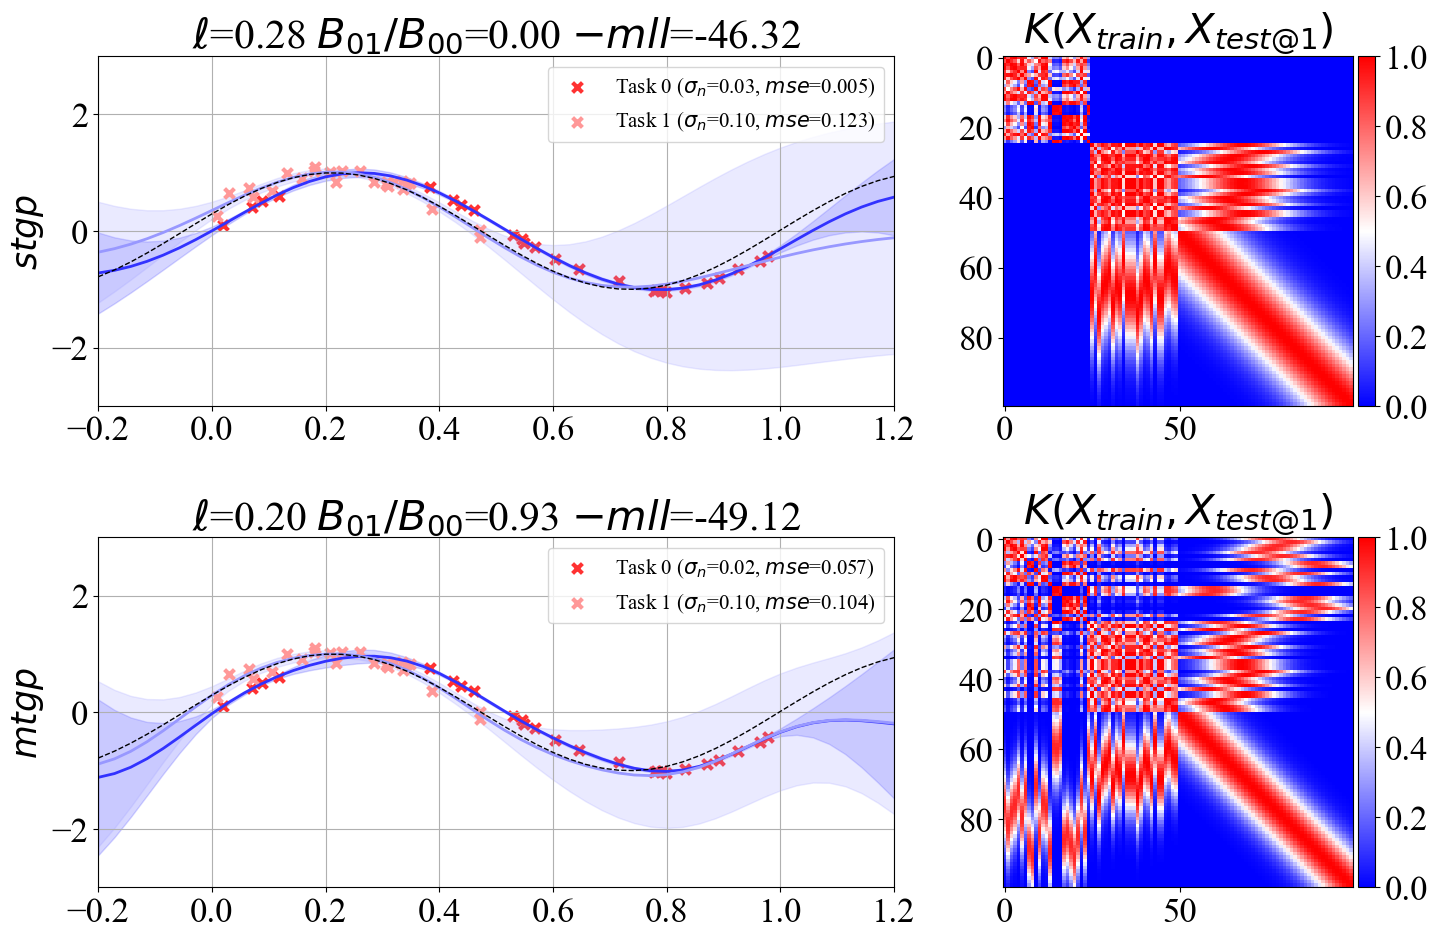
\includegraphics[width=\textwidth]{assets/plt_mtgp_coorperative.png}
    \caption{Observations for the two tasks are generated $y_0(x)=\sin(6x) + .03 \epsilon$ and $y_1(x)=\sin(6x + \texttt{shift}) + .1 \epsilon$ where $\epsilon\overset{iid}{\sim} \sN(0,1)$ and $\texttt{shift}=.3$. Here for task 1 we only sample points in $[0,.5]$ while for task 0 we sample points in $[0,1]$. (Top) Two Gaussian process regressor are learnt to fit data independently. (Bottom) A MTGP is fit to data whereby the task similarity matrix $B:=K^t$ is learnt by maximizing marginal log likelihood. We see that by taking into account of relationship between tasks, samples from task 0 reduces uncertainty that task 1 has at test locations far from its training support.}
    \label{fig:plt_mtgp_coorperative}
\end{figure}
\end{center} 

\begin{center} 
\begin{figure}[h!]
    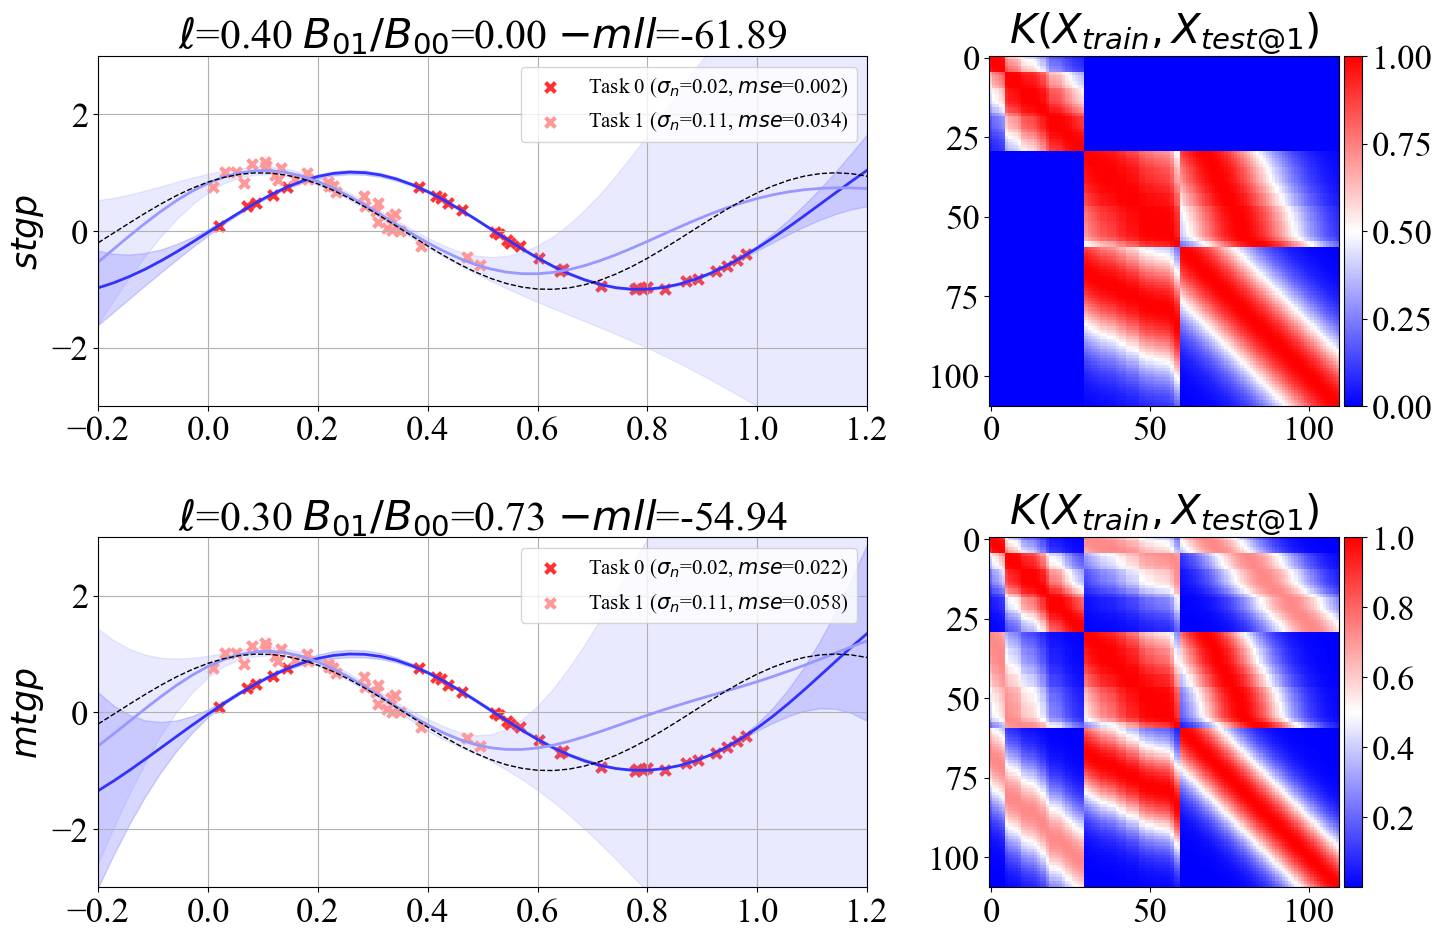
\includegraphics[width=\textwidth]{assets/plt_mtgp_competitive.png}
    \caption{Observations for the two tasks are generated $y_0(x)=\sin(6x) + .03 \epsilon$ and $y_1(x)=\sin(6x + \texttt{shift}) + .1 \epsilon$ where $\epsilon\overset{iid}{\sim} \sN(0,1)$ and  and $\texttt{shift}=1.5$. Here for task 1 we only sample points in $[0,.5]$ while for task 0 we sample points in $[0,1]$. There are 4 times training points for task 0 than task 1 (Top) Two Gaussian process regressor are learnt to fit data independently. (Bottom) A MTGP is fit to data whereby the task similarity matrix $B:=K^t$ is learnt by maximizing marginal log likelihood. We see in case of data imbalance, which often happens in multitask learning, we arrive at an optimal marginal likelihood for all data points (a larger marginal likelihood), but renders prediction suboptimal for task 1 (a higher MSE)}
    \label{fig:plt_mtgp_competitive}
\end{figure}
\end{center} 

    

\subsection{Asymmetric MTGP}

When the goal is to improve performance of a target/main task given the other tasks, optimizing for maximum marginal likelihood of all tasks is suboptimal, as shown in Figure~(\ref{fig:plt_mtgp_competitive}). There are extension of MTGP to the asymmetric case by assuming that auxiliary task functions are addition of a shared main task function and task specific function \cite{leenFocusedMultitaskLearning2012}, however it still uses the full marginal likelihood for all tasks to find task similarity and kernel hyperparameters. Ideally, we want
\begin{enumerate}
    \item An objective which depends on likelihood of main task only
    \item Automatically learn the task similarity such that auxiliary task or side information can improve learning of main task. If a side task is totally unrelated to the main task, it should have minimal influence on learning of the main task.
\end{enumerate}
Given design $X\in\R^{N\times D}, Y\in \R^{N\times 1}, S\in\R^{N\times M}$, we want to learn a scalar valued regressor $f:\R^D \to \R$ that fits the data well. We can alternatively try to learn the scalar valued regressor taking into account of relevant side information $f:\R^D\times \R^M \to\R$. Relevant side information that helps with learning the main task should be selected from potentially irrelevant side information. A simple thing one can do is to define a kernel that captures similarity between inputs via $k_x$ and similarity of side information $k_s$, similar to the setup of MTGP. Let $k$ be a tensor product $k_x\otimes k_s$ over $\sX\times \sS$, 
\begin{align}
    k((x,s),(x',s'))
        = k_x(x,x') k_s(s,s')
    \label{eq:amtgp_product_kernel}
\end{align}
Instead of task similarity matrix, correlation between any pair $y,y'$ depends on value of $k_s(s,s')$. In the case where $s$ describes a particular sub-population of our training dataset, it gives rise to a stratification dependent kernel. In health care domain, we might want to provide stratification dependent predictions given our side information of scanner, patient orientation, and existence of comorbidities. In this setting, automatic selection of relevance can be achieved via an Automatic Relevance Determination (ARD) kernel
\begin{align}
    k_s(s,s')
        = \sigma^2 \exp\left(
            -\frac{1}{2} \sum_{l=1}^M \frac{1}{\ell_l^2} (s_l - s'_l)^2 
        \right)
    \label{eq:amtgp_ard_kernel}
\end{align}
If ARD kernel is used, current formulation captures the prior that main task regressor is smooth with respect to some stratification of dataset - at test time the model will give similar prediction to those that appears to be likely in the same training stratification, as shown in Figure (\ref{fig:plt_amtgp_shift=0.0_scale=12}). Hyperparameters $\pc{\pc{\ell_l}_{l=1}^M, \theta_{k_x}}$ can be learnt by maximizing marginal likelihood. 

One complication is missing side information during training, no information exists for some components of $s$. A more serious issue is at test time, we would want our parameterized function $f$ to make prediction based on $x_*$ only, absent of any side information. Naively this is not possible, since our regressor is supported over $\sX\times\sS$. A easy way to fix this is to pre-train a model with the goal of predicting side information from $x$ - we first impute the missing side information, then proceed with both training and testing. A more principled way to do this is to train some GP model and use its predictive distribution over the side information as inputs for training and testing of $f$. This is related to GP with uncertain inputs and there is closed form solution for inference. 

For a toy case where $D=1,M=1$, we see that the asymmetric MTGP described just now is able to utilize side information when they help Figure (\ref{fig:plt_amtgp_shift=0.0}) and ignore side information when they are irrelevant Figure (\ref{fig:plt_amtgp_shift=1.0}). A summary of model performance for main task regressor with varying side information relevance is in Table (\ref{table:amtgp_mse_wrt_shift}). A summary of how much \texttt{amtgp} depends on side information is in Table (\ref{table:amtgp_lengthscale_ratio}). 

\begin{table}[h!]
\begin{center}
    \begin{tabular}{r|rrr}
        \texttt{shift} &  \texttt{stgp} &   \texttt{mtgp} &   \texttt{amtgp} \\
    \hline
        0.000 &  0.579 &  0.021 &   0.181 \\
        0.100 &  0.660 &  0.030 &   0.106 \\
        0.200 &  0.735 &  0.026 &   0.088 \\
        0.300 &  0.802 &  0.027 &   0.162 \\
        0.400 &  0.857 &  0.041 &   0.246 \\
        0.500 &  0.898 &  0.070 &   0.256 \\
        1.000 &  0.837 &  0.139 &   0.296 \\
    \end{tabular}
    \caption{Mean squared error for main task (task=1) regressor at test locations along the grid ($\texttt{linspace}$(0,1,100)) for the three different methods \texttt{stgp},\texttt{mtgp},\texttt{amgtp} trained on data of varying task similarity. Larger values of \texttt{shift} implies the two task functions are more unrelated. \texttt{mtgp} is more flexible than \texttt{stgp} and therefore gives a higher marginal likelihood assuming the task similarity matrix can be found properly. \texttt{amtgp} is able to utilize side information when they are really relevant $\texttt{shift}=0$, and does not suffer from performance drop when the two tasks are irrelevant $\texttt{shift}=1.0$ }
    \label{table:amtgp_mse_wrt_shift}
\end{center}
\end{table}

\begin{table}[h!]
\begin{center}
    \begin{tabular}{r|r}
        \texttt{shift} &   $\frac{\ell_s}{\ell_x}$ \\
    \hline
            0.0 &     0.1 \\
            0.1 &     0.7 \\
            0.5 &     8.8 \\
            1.0 &    23.4 \\
            1.5 &    29.4 \\
    \end{tabular}
    \caption{Ratio of lengthscale for $k_s$ over length scale for $k_x$, e.g. $\frac{\ell_s}{\ell_x}$ for main task (task=1) regressor trained via \texttt{amtgp}. A larger ratio implies the model relies more on $x$ and less on side information $s$}
    \label{table:amtgp_lengthscale_ratio}
\end{center}
\end{table}



\begin{center} 
\begin{figure}[h!]
    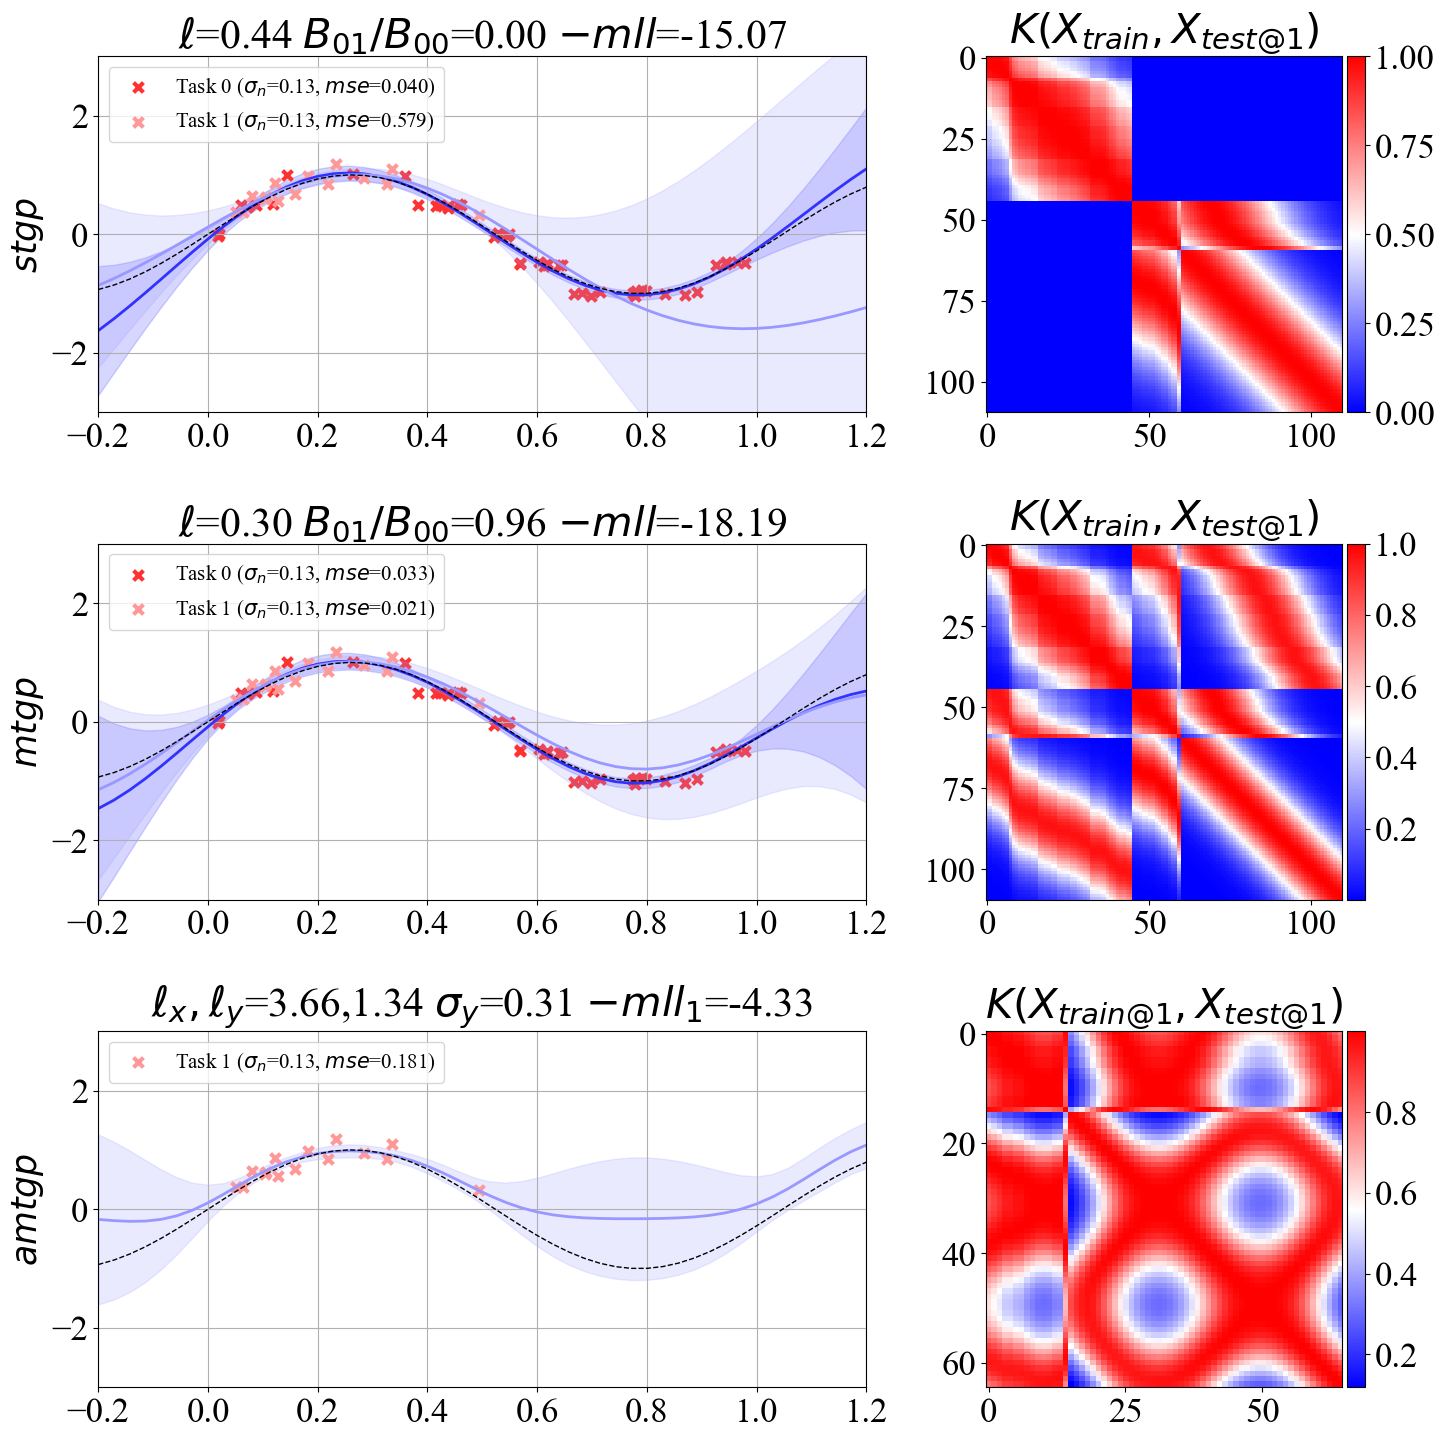
\includegraphics[width=\textwidth]{{{assets/plt_amtgp_shift=0.0}}}
    \caption{(Top) \texttt{stgp} GP regressors are learnt independently (Middle) \texttt{mtgp} GP regressors learnt via MTGP (Bottom) \texttt{amtgp} GP regressor for task 1 (main task) where the GP prior has kernel defined in Equation (\ref{eq:amtgp_product_kernel}, \ref{eq:amtgp_ard_kernel}). Missing side information is imputed from the predictive mean of a pre-trained \texttt{stgp} GP regressor for task 0. Bandwidth for the squared exponential kernel $k_x$ and ARD kernel $k_s$, e.g. $\pc{\ell_x, \ell_s}$, is optimized by maximizing the marginal likelihood of task 1 data points. We see, in case where the tasks are related, as measured by a large $\texttt{shift}=0.$ betwen these two task functions. We see \texttt{mtgp} is able to utilize side information really effectively while \texttt{amtgp} also learns to rely on side information, as seen from a small $\ell_s$, and reduce its uncertainty of prediction far away from its training support. }
    \label{fig:plt_amtgp_shift=0.0}
\end{figure}
\end{center} 
    

 

\begin{center} 
\begin{figure}[h!]
    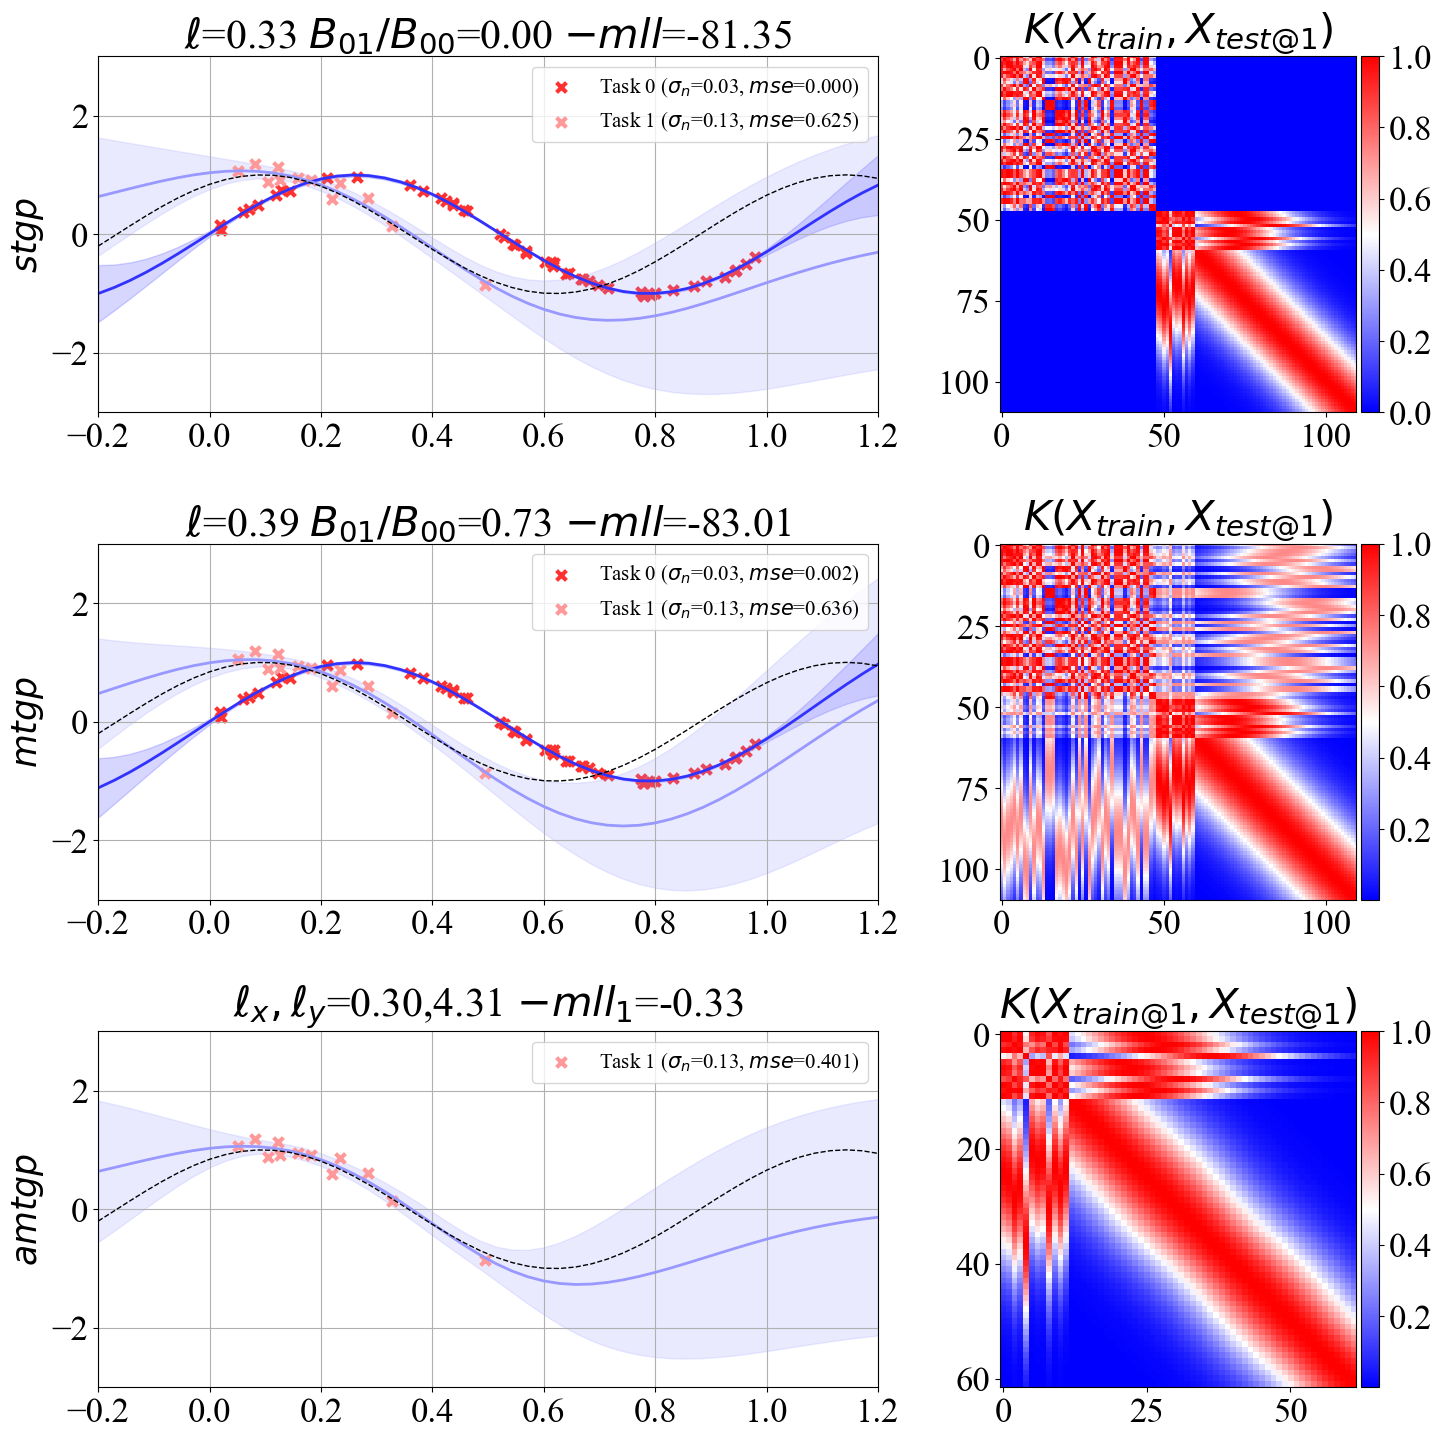
\includegraphics[width=\textwidth]{{{assets/plt_amtgp_shift=1.0}}}
    \caption{(Top) \texttt{stgp} GP regressors are learnt independently (Middle) \texttt{mtgp} GP regressors learnt via MTGP (Bottom) \texttt{amtgp} GP regressor for task 1 (main task) where the GP prior has kernel defined in Equation (\ref{eq:amtgp_product_kernel}, \ref{eq:amtgp_ard_kernel}). Missing side information is imputed from the predictive mean of a pre-trained \texttt{stgp} GP regressor for task 0. Bandwidth for the squared exponential kernel $k_x$ and ARD kernel $k_s$, e.g. $\pc{\ell_x, \ell_s}$, is optimized by maximizing the marginal likelihood of task 1 data points. We see, in case where the tasks are unrelated and perhaps even conflicting, as measured by a large $\texttt{shift}=1.0$ between these two task functions, we see \texttt{mtgp} prediction is more uncertain in regions where task 1 function is supported and task 0 function is not. This is a result of \texttt{mtgp} able to use data points from task 0 observations even if the two functions are unrelated. \texttt{amtgp} learns to ignore side information as seen from large values of $\ell_s$, and reduces to \texttt{stgp} regression}
    \label{fig:plt_amtgp_shift=1.0}
\end{figure}
\end{center} 


    


\begin{center} 
\begin{figure}[h!]
    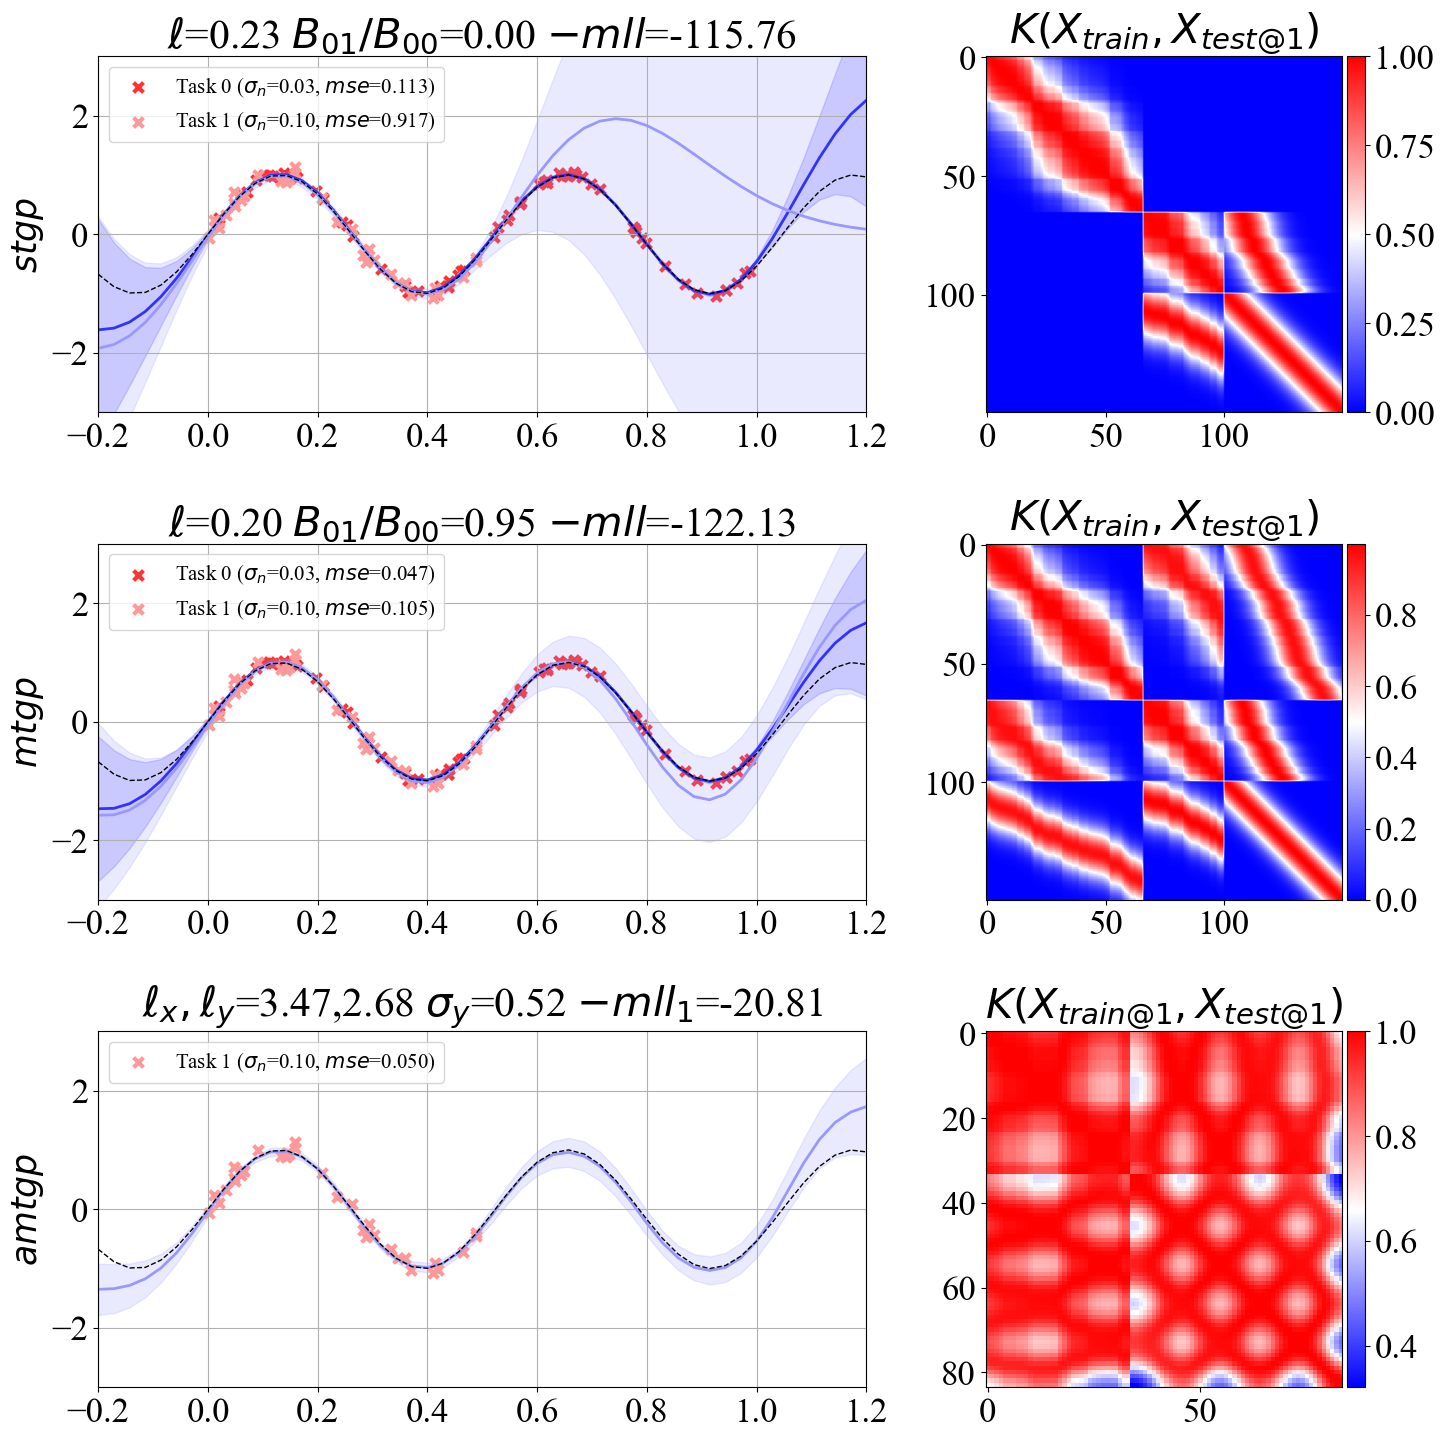
\includegraphics[width=\textwidth]{{{assets/plt_amtgp_shift=0.0_scale=12}}}
    \caption{(Top) \texttt{stgp} GP regressors are learnt independently (Middle) \texttt{mtgp} GP regressors learnt via MTGP (Bottom) \texttt{amtgp} GP regressor for task 1 (main task) where the GP prior has kernel defined in Equation (\ref{eq:amtgp_product_kernel}, \ref{eq:amtgp_ard_kernel}). We see \texttt{amtgp} can extrapolate training support by utilizing prediction of side task.}
    \label{fig:plt_amtgp_shift=0.0_scale=12}
\end{figure}
\end{center} 



\newpage
\printbibliography 




\end{document}